\documentclass[openany]{book}
\usepackage[utf8]{inputenc}
\usepackage[english]{babel}
\usepackage{graphicx}
\usepackage{enumerate}
\usepackage{float}
\graphicspath{ {} }
\usepackage{mathtools}
\usepackage{amsmath, amsthm, amssymb, amsfonts}
\usepackage{caption}
\usepackage{fancyhdr}
\pagestyle{fancy}
\fancyhf{}
\rhead{Ty Darnell}
\lhead{Final Notes}
\usepackage{hyperref}
\hypersetup{
	colorlinks=true,
	linkcolor=blue,
	filecolor=magenta,      
	urlcolor=cyan,
	pdftitle={Bios * Notes},
	pdfauthor={Ty Darnell},
	bookmarksopen=true,
}
% For derivatives
\newcommand{\deriv}[1]{\frac{\mathrm{d}}{\mathrm{d}x} (#1)}

% For partial derivatives
\newcommand{\pderiv}[2]{\frac{\partial}{\partial #1} (#2)}

% Integral dx
\newcommand{\dx}{\mathrm{d}x}
\begin{document}
\tableofcontents
\chapter{Distributions}
\section{Bernoulli}
$p^x(1-p)^{1-x} \quad x=0,1$\\
$EX=p \quad VarX=p(1-p)$
\section{Poisson}
Expresses the probability of a given number of events occuring during a fixed interval of time or space if these events occur with a known constant rate independently of the time since the last event.\\
$\dfrac{\lambda^x e^{-\lambda}}{x!}$\medbreak
$EX=\lambda \quad VarX= \lambda$
\section{Geometric}
The probability distribution of the number X of bernoulli trials needed to get one success.\\
$(1-p)^{x-1}p \quad x=1,\dots$\\
$1-(1-p)^x$\medbreak
$EX=\dfrac{1}{p} \quad VarX=\dfrac{1-p}{p^2}$
\section{Binomial}
distribution of the number of successes in a sequence of n independent bernoulli trials.\\
$\binom{n}{x} p^x(1-p)^{n-x}$ \medbreak
$EX=np \quad VarX=np(1-p)$
\section{Negative Binomial}
number of successes in a sequence of iid bernoulli trials before a specified number of failures (r).\\
$\binom{k+r-1}{k}(1-p)^r p^k$\medbreak
Negative Binomial Mgf $\left(\dfrac{p}{1-(1-p)e^t}\right)^r$\\
$EX=\dfrac{r(1-p)}{p} \quad VarX=\dfrac{r(1-p)}{p^2}$
\section{Hypergeometric}
The result of each draw (the elements of the population being sampled) can be classified into two mutually exclusive categories ie pass/fail.\\
The probability of a success changes on each draw, as each draw decreases the population (sampling without replacement from a finite population)\\
N=population size\\
M=number of success in the population\\
K= number of draws\\
x=number of observed successes\\
$\dfrac{\binom{M}{x}\binom{N-M}{K-x}}{\binom{N}{K}}$\\
$EX=\dfrac{KM}{N} \quad VarX= \dfrac{KM}{N}\dfrac{(N-M)(N-K)}{N(N-1)}$
\section{Exponential}
describes the waiting time between Poisson events, Memoryless\\
$\lambda e^{-\lambda x} \quad 0\leq x<\infty \quad \lambda>0$\\
$1-e^{-\lambda x}$\medbreak
$EX=\dfrac{1}{\lambda} \quad VarX=\dfrac{1}{\lambda^2}$
\section{Normal}
$\dfrac{1}{\sqrt{2\pi}\sigma}e^{-\dfrac{(x-\mu)^2}{2\sigma^2}}$\\
$EX=\mu \quad VarX=\sigma^2$
\section{Uniform}
\subsection{Uniform Continuous}
symmetric probability distribution where all intervals of the same length are equally probable.\\
$\dfrac{1}{b-a}$\\
$\dfrac{x-a}{b-a}$\medbreak
$EX=\dfrac{b+a}{2} \quad VarX=\dfrac{(b-a)^2}{12}$
\subsection{Uniform Discrete}
a symmetric probability distribution where a finite number of values are equally likely to be observed. Every one of n values has an equal probability 1/n.\\
$\dfrac{1}{n} \quad x=1,\dots,N \quad N=1,\dots$\medbreak
$EX=\dfrac{N+1}{2} \quad VarX=\dfrac{(N+1)(N-1)}{12}$
\section{Gamma Distribution}
Gamma Function: $\Gamma(\alpha)=\int_{0}^{\infty}t^{\alpha-1}e^{-t} \ dt$\\
$\Gamma(\alpha+1)=\alpha \Gamma(\alpha) \ \alpha>0$\\
$\Gamma(n)=(n-1)! \quad n \in \mathbb{Z}$\\
$\Gamma(1/2)=\sqrt{\pi}$\\
$f(x|\alpha,\beta)=\dfrac{1}{\Gamma(\alpha) \beta^\alpha}x^{\alpha-1}e^{-x/\beta}$\\
$\alpha$ is the shape parameter, influences the peakedness of the distribution\\
$\beta$ is the scale parameter, influences the spread of the distribution\\
$EX^v=\dfrac{\beta^v \Gamma(v+\alpha)}{\Gamma(\alpha)}$\\
$\Gamma(\alpha+v)=\int_{0}^{\infty}x^{v+\alpha-1}e^{-x} \ \dx$\\
$EX=\alpha \beta$ alternatively $a/\lambda$ $\lambda=1/\beta$\\
$Var(X)=ab^2$ alternatively $a/\lambda^2$\\
$\int_{0}^{\infty}e^{-x^2/2} \ dz=\dfrac{\sqrt{2\pi}}{2}=\sqrt{\dfrac{\pi}{2}}$\\
$\int_{0}^{\infty}x^2e^{-x^2}$ is the same\\
\section{Beta Distribution}
$f(x|\alpha,\beta)=\dfrac{1}{B(\alpha,\beta)}x^{\alpha-1}(1-x)^{\beta-1} \quad 0\leq x\leq 1$\\
Beta Function: $B(\alpha,\beta)=\int_{0}^{1}x^{\alpha-1}(1-x)^{\beta-1} \ \dx$ \\ 
$B(\alpha,\beta)=\dfrac{\Gamma(\alpha)\Gamma(\beta)}{\Gamma(\alpha+\beta)}$\\
$EX^n=\dfrac{B(\alpha+n,\beta)}{B(\alpha,\beta)}=\dfrac{\Gamma(\alpha+n)\Gamma(\alpha+\beta)}{\Gamma(\alpha+\beta+n)\Gamma(\alpha)}$\\
$E(X)=\dfrac{a}{a+b}$\\
$Var(X)=\dfrac{ab}{(a+b)^2(a+b+1)}$\\
$beta(1,1)=U(0,1)$
\section{Mgfs}
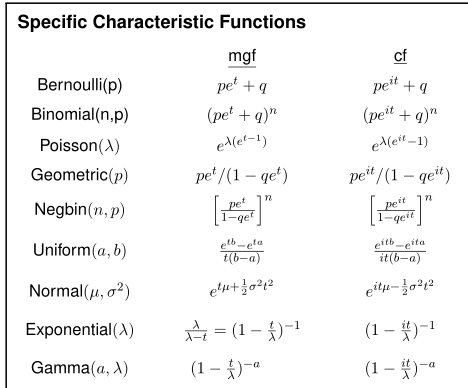
\includegraphics[scale=1]{mgfchar.png}
\section{Location and Scale Families}
\[f_{\mu,\sigma}(x)=\dfrac{1}{\sigma}f\left(\dfrac{x-\mu}{\sigma} \right)
\]
$\mu \in \mathbb{R} \quad \sigma>0$ is a location scale family\\
If $\mu=0$ scale family\\
If $\sigma=1$ location family\\
Properties: Let $Z\sim f(z)$ and $X=\sigma Z+\mu$ Then\\
X has pdf $f_{\mu,\sigma}$\\
$E(X)=\sigma E(Z)+\mu \quad Var(X)=\sigma^2 Var(Z)$

\chapter{Notes 13}
\section{Conditional Probability}
\[f(y|x)=\dfrac{f(x,y)}{f(x)}
\]
\section{Exponential Families}
A family of pdfs or pmfs is called an exponential family if it can be expressed as
\[f(x|\theta)=h(x)c(\theta)\exp\left(\sum_{i=1}^{k}w_i(\theta)t_i(x)\right)
\]
\section{Multinomial Distribution}
$p(s_1,s_2,\dots,s_k)=\dfrac{n!}{s_1!s_2!\dots s_k!}p_1^{s_1}p_2^{s_2}\cdots p_k^{s_k}$\\
where $\sum_{i=1}^{k}s_1=n$ and $\sum_{i=1}^{k}p_i=1$\\

\chapter{Notes 14}
\section{Convolution}
If X and Y are independent continuous r.v.s with pdfs $f_X(x)$ and $f_Y(y)$, then the pdf of $Z=X+Y$ is:
\[f_Z(z)=\int_{-\infty}^{\infty}f_X(w)f_Y(z-w)\ dw
\]
\section{Sum of Two Independent Poissons}
$X\sim Pois(\lambda_1), \ Y\sim Pois(\lambda_2)$\\
$U=X+Y \ V=Y$\\
$X=U-V \ Y=V$\\
Joint PMF of U and V is:\\
$f_{U,V}(u,v)=f_{X,Y}(u-v,v)=\dfrac{e^{-\lambda_1}\lambda_1^{u-v}}{(u-v)!}\dfrac{e^{-\lambda_2}\lambda_2^v}{v!}$\\
The distribution of $U=X+Y$ is the marginal:\\
$f_U(u)=\sum_{v=0}^{u}\dfrac{e^{-\lambda_1}\lambda_1^{u-v}}{(u-v)!}\dfrac{e^{-\lambda_2}\lambda_2^v}{v!}$\\
$=\dfrac{e^{-(\lambda_1+\lambda_2)}}{u!}\sum_{v=0}^{u} {u \choose v}\lambda_1^{u-v}\lambda_2^v$\medbreak
Because of the binomial theorem\medbreak
$=\dfrac{e^{-(\lambda_1+\lambda_2)}}{u!}(\lambda_1+\lambda_2)^u$\medbreak
$U\sim Pois(\lambda_1+\lambda_2)$
\section{Jacobian}
$J(u,v)$ is the Jacobian of the transformation $(x,y)\to (u,v)$ given by:\medbreak
$J(u,v)=\dfrac{\partial(x,y)}{\partial(u,v)}=
\begin{bmatrix}
\dfrac{\partial x}{\partial u}& \dfrac{\partial x}{\partial v}\\
\dfrac{\partial y}{\partial u}& \dfrac{\partial y}{\partial v}\\
\end{bmatrix}$
\section{Functions of Independent Random Variables}
Let X and Y be independent r.v.s\\
Let $g:\mathbb{R}\to \mathbb{R}$ and $h:\mathbb{R}\to \mathbb{R}$ be functions\\
Then the r.v.s $U=g(X)$ and $V=h(Y)$ are independent
\section{Ratio of Two Independent Normals}
Let $X \sim N(0,1)$ and $Y\sim N(0,1)$\\
The ratio $X/Y$ has the Cauchy distribution\\
Let $U=X/Y$ and $V=Y$ \quad Then $X=UV$ and $Y=V$ \quad $J(u,v)=v$\\
$f_{X,Y}(x,y)=\dfrac{1}{\sqrt{2\pi}}e^{-x^2/2}\dfrac{1}{\sqrt{2\pi}}e^{-y^2/2}=\dfrac{1}{2\pi}e^{-(x^2+y^2)/2}$\\
$f_{U,V}(uv,v)=\dfrac{1}{2\pi}e^{-[(uv)^2+v^2]/2}*|v|=\dfrac{|v|}{2\pi}e^{-(u^2+1)v^2/2}$\\
$f_{U}(u)=\int_{-\infty}^{\infty}f_{UV}(u,v) \ dv=2\int_{0}^{\infty}\dfrac{v}{2\pi}e^{-(u^2+1)v^2/2} \ dv$\\
$=\dfrac{1}{\pi}\int_{0}^{\infty}e^{-(u^2+1)z} \ dz=\dfrac{1}{\pi(u^2+1)}$
\section{Sum of Two Independent Random Variables}
Suppose X and Y are independent, find distribution of $Z=X+Y$\\
In general: $F_Z(z)=P(X+Y\leq z)=P(\{(x,y) \text{ such that } x+y\leq z\})$\\
Approaches:
\begin{itemize}
\item Bivariate transformation method (continuous and discrete)\\
\item Discrete convolution:\\
$f_Z(z)=\sum_{x+y=z}f_X(x)f_Y(y)=\sum_{x}f_X(x)f_Y(z-x)$\\
\item Continuous convolution\\
\item Mgf/cf method (continuous and discrete)\\
$\phi_Z{\theta}=\phi_X(\theta)\phi_Y(\theta)$\\
$Z=X-Y \quad \phi_Z{\theta}=\phi_X(\theta)\phi_Y(-\theta)$
\end{itemize}
\chapter{Notes 15}
\section{Conditional Expectation and Variance}
For two r.v.s X and Y with conditional pdf $f_{Y|X}(y|x)$ the conditional expectation of $g(Y)$ give $X=x$ is:\\
$h(x)=E[g(Y)|x]=\int_{-\infty}^{\infty}g(y)f_{Y|X}(y|x) \ dy$\\
$h(X)=E[g(Y)|X]$\\
\textbf{Iterative Expectation Formula}\\
$EX=E(E(X|Y))$\\
\textbf{Variance}\\
$Var[g(Y)]=E[g(y)-E(g(Y))]^2$\medbreak
$VarX=E(Var(X|Y))+Var(E(X|Y))$\\
$Var(g(Y)|X)=E\{[g(Y)-E(g(Y)|X)]^2|X\}$\\
where both expectations are taken with respect to $f_{Y||X}(y)$\\
\begin{itemize}
\item $E(Var(X|Y))=E\{[X-E(X|Y)]^2\}$\\
\item $Var(E(X|Y))=E\{[E(X|Y)-EX]^2\}$\\
\end{itemize}
\section{Covariance and Correlation}
$Cov(X,Y)=E[(X-\mu_X)(Y-\mu_Y)]=\sigma_{XY}$\\
Correlation =$\rho_{XY}=\dfrac{Cov(X,Y)}{\sqrt{VarX \ VarY}}=\dfrac{\sigma_{XY}}{\sigma_X \sigma_Y}$\\
$=E\left[ \left( \dfrac{X-\mu_X}{\sigma_X} \right) \left( \dfrac{Y-\mu_Y}{\sigma_Y} \right) \right]$\medbreak
X and Y are uncorrelated iff:\\
$Cov(X,Y)=0$ or equivalently $\rho_{XY}=0$\\
$Cov(X,Y)=E(XY)-E(X)E(Y)$\\
If X and Y are independent and $Cov(X,Y)$ exists, then $Cov(X,Y)=0$\\
If X and Y are uncorrelated this does not imply independence.\\
\section{Linear Combinations}
$Cov(aX+B_Y,Z)=aCov(X,Z)+bCov(Y,Z)$\medbreak
$Var(aX+bY)=a^2Var(X)+b^2Var(Y)+2abCov(X,Y)$\medbreak
$Corr(aX+b,cY+d)=\dfrac{ac}{|ac|}Corr(X,Y)$
\section{Standard Bivariate Normal}
$f_{XY}(x,y)=\dfrac{1}{2\pi\sqrt{1-\rho^2}}\exp{\left[-\dfrac{x^2-2\rho xy+y^2}{2(1-\rho^2)}\right]}$\\
Both X and Y have marginal distributions are $N(0,1)$\\
Correlation of X and Y is $\rho$\\
Conditional Distribution are normal:\\
$Y|X \sim N(\rho X,1-\rho^2) \quad X|Y \sim N(\rho Y, 1-\rho^2)$\\
The means are the regression lines of Y on X and X on Y respectively.
\section{Bivariate Normal}
Let $\tilde{X}$ and $\tilde{Y}$ have a standard bivariate normal distribution with correlation $\rho$\\
Let $X=\mu_X+\sigma_X\tilde{X} \quad Y=\mu_Y+\sigma_Y\tilde{Y}$\\
Then $(X,Y)$ has the bivariate normal density:\\
$f_{XY}(x,y)=\left(2\pi \sigma_X \sigma_Y \sqrt{1-\rho^2} \right)^{-1}\exp{\left\{-\dfrac{1}{2(1-\rho^2)}\left[\left(\dfrac{x-\mu_X}{\sigma_X} \right)^2- 2\rho \left(\dfrac{x-\mu_X}{\sigma_X} \right)\left(\dfrac{y-\mu_Y}{\sigma_Y} \right)+\left(\dfrac{y-\mu_Y}{\sigma_Y} \right)^2 \right] \right\}}$\medbreak
Marginal distributions: $N(\mu_X,\sigma^2_X) \quad N(\mu_Y,\sigma^2_Y)$\\
$Corr(X,Y)=\rho$\medbreak
Conditional distributions are normal:\\
$Y|X \sim N[\mu_Y+\rho(\sigma_Y/\sigma_X)(x-\mu_X),\sigma^2_Y(1-\rho^2)]$\medbreak
Distribution of $aX+bY$ is:\\
$N(a\mu_X+b\mu_Y,a^2\sigma^2_X+b^2\sigma^2_Y+2ab\rho \sigma_X \sigma_Y)$
\section{Multivariate Distributions}
$\boldsymbol{X}=(X_1,X_2,\dots, X_n)$\\
If $\boldsymbol{X}$ is discrete then:\\
$P(\boldsymbol{X} \in A)=\sum_{\boldsymbol{X} \in A} f(\boldsymbol{X})$\\
where $f(\boldsymbol{X})$ is the joint pmf\\
If $\boldsymbol{X}$ is continuous then:\\
$P(\boldsymbol{X}\in A)=\int \cdots \int_{A}f(x_1,\dots,x_n)dx_1,\dots dx_n$\medbreak
\section{Marginals and Conditionals}
The \textbf{marginal} pdf or pmf of any subset of coordinates is found by integrating or summing the joint pdf or pmf over all possible values of the other coordinates.\medbreak
The \textbf{conditional} pdf or pmf of a subset of coordinates given the values of the remaining coordinates is found by dividing the full joint pdf or pmf by the joint pdf or pmf of the remaining variables.
\section{Multivariate Independence}
Independent Random Vectors:\\
Let $\boldsymbol{X_1},\dots,\boldsymbol{X_n}$ be random vectors with joint pdf or pmf $f(\boldsymbol{X_1},\dots,\boldsymbol{X_n})$\\
Let $f\boldsymbol{X_j}(\boldsymbol{x_j})$ be the marginal pdf or pmf of $\boldsymbol{X_j}$.\\
Then $\boldsymbol{X_1},\dots,\boldsymbol{X_n}$ are \textbf{mutually independent} random vectors if:\\
$\forall$ $(\boldsymbol{X_1},\dots,\boldsymbol{X_n})$: \quad  $f(\boldsymbol{X_1},\dots,\boldsymbol{X_n})=\prod_{j=1}^{n}f\boldsymbol{X_j}(\boldsymbol{x_j})$
\section{Multinomial}
Let n and m be positive integers and let $p_1,\dots,p_n$ be probabilities summing to one. Then the random vector $(X_1,\dots,X_n)$ has a multinomial distribution with m trials and cell probabilities $p_1,\dots,p_n$ if its joint pmf is:
\begin{align*}
f(x_1,\dots,x_n)&={m \choose x_1,\cdots,x_n} p_1^{x_1}\cdots p_n^{x_n}\\
&=\dfrac{m!}{x_1! \dots x_n!}p_1^{x_1}\cdots p_n^{x_n}\\
&= m!\prod_{j=1}^{n}\dfrac{p_j^{x_j}}{x_j!}
\end{align*}
for $x_1=0,\dots,m \quad i=1,\dots,n \quad x_1+\cdots+x_n=m$
\chapter{Notes 16}
\section{Inequalities}
\textbf{Chebychev Inequality}\\
$P[g(X)\geq r] \leq \dfrac{E[g(X)]}{r}$\\
If X is nonnegative and g is a positive non-decreasing function then:\\
$P\{X\geq a \}\leq \dfrac{E[g(X)]}{g(a)}$\\
\textbf{Special Cases:}\\
$X\geq 0$ \quad $P\{X\geq a \}\leq \dfrac{E(e^{tX})}{e^{ta}}$\\
$L^p$ Space- consists of all r.v.s whose $p^{th}$ absolute power is integrable, $E(|X|^p)<\infty$\\
\textbf{Triangle Inequality}\\
$|a+b|\leq |a|+|b|$\\
\textbf{Convex Functions}\\
A function $g: I\to R$ is convex for any $\lambda \in [0,1]$ and any points x and y in I\\
$g[\lambda x+(1-\lambda)y]\leq \lambda g(x)+(1-\lambda)g(y)$\\
A differentiable function g is convex iff it lays above all tangents.\\
A twice differentiable function g is convex iff its second derivative is non-negative\\
concave if -g is convex on I\\
\textbf{Jensen's Inequality}\\
Let $X \in L^1$ and $g(x)$ be a convex function where $E[g(X)]$ exists. Then:\\
$E[g(X)]\geq g[EX]$\\
with equality iff for every line $a+bx$ tangent to $g(x)$ at $x=EX, P[g(X)=a+bX]=1$\\
direction of inequality is reversed if g is concave\\
\textbf{Young's Inequality}\\
Let $a,b >0$ and $p,q>1$ with $1/p+1/q=1$ Then:\\
$\dfrac{a^p}{p}+\dfrac{b^q}{q}\geq ab$\\
with equality iff $a^p=b^q$\\
\textbf{Holder's Inequality}\\
Suppose $X \in L^p, Y \in L^q$ where $p,q>1$ and $1/p+1/q=1$ Then:\\
$E[|XY|]\leq [E|X|^p]^{1/p}E[|Y|^q]^{1/q}$\\
with equality if $X^p=cY^q$ for some $c \in \mathbb{R}$\\
\textbf{Cauchy-Schwartz Inequality}\\
corollary of Holders where $p=q=2$\\
$E[|XY|]\leq [E|X|^2]^{1/2}E[|Y|^2]^{1/2}=\sqrt{E[X^2]E[Y^2]}$\\
with equality if $X=cY$\\
\textbf{Lyapunov's Inequality}\\
corrallary of Holders\\
for $1\leq r\leq s$ and $X\in L^s$\\
$E[|X|^r]^{1/r}\leq E[|X|^s]^{1/s}$\\
\textbf{Application of Cauchy-Schwartz}\\
$p=\dfrac{Cov(X,Y)}{\sqrt{Var(X)Var(Y)}}$\\
Then $|p|\leq 1$ with equality iff $Y-\mu_Y=c(X-\mu_X)$\\
\textbf{Minkowski's Inequality}\\
Suppose $X,Y \in L^p, p\geq 1$ Then $(X+Y)\in L^p$ and\\
$[E|X+Y|^p]^{1/p}\leq [E|X|^p]^{1/p}+[E|Y|^p]^{1/p}$\\
\section{Order Statistics}
\textbf{Distribution of the Maximum}\\
The cdf of $Z=max(Y_1,\dots,Y_n)$ is\\
\begin{align*}
F_Z(z)&= P\{Z\leq z \}\\
&=P\{Y_1\leq z, Y_2 \leq z,\dots, Y_n \leq z \}\\
&=\prod_{j=1}^{n}P\{Y_j\leq z \} \text{ indep}\\
&=F_Y(z)^n \text{ ident. distrib}
\end{align*}
Thus the pmf is:\\
$f_Z(z)=nF_Y(z)^{n-1}f_Y(z)$\\
\textbf{Distribution of the Minimum}\\
$W=min(Y_1,\dots,Y_n)$\\
$F_W(w)=1-(1-F_Y(w))^n$\\
$f_W(w)=n(1-F_Y(w))^{n-1}f_Y(w)$\\
\textbf{Order Statistics}\\
Let $Y_1,Y_2,\dots, Y_n$ be iid with pdf $f_Y(x)$\\
Order the observations:\\
$Y_{(1)}\leq Y_{(2)}\leq \cdots \leq Y_{(n)}$\\
The $Y_{(i)}$ are called order statistics. Minimum is $Y_{(1)}$ max is $Y_{(n)}$\\
We are interested in finding the distribution of an arbitrary $Y_{(i)}$ as well as the joint distributions of sets of $Y_{(i)}$s and $Y_{(j)}$s\\
ex: Range=$Y_{(n)}-Y_{(1)}$\\
$r^{th}$\textbf{ order statistic}\\
We need to find the density of $Y_{(r)}$ at a value y\\
Consider 3 intervals $(-\infty,y),[y,y+dy),[y+dy,\infty)$\\
The number of observations in each of the intervals follows the tri-nomial distribution:\\
$f(s_1,s_2,s_3)=\dfrac{n!}{s_1!s_2!s_3!}p_1^{s_1}p_2^{s_2}p_3^{s_3}$\\
The event that $y\leq Y_{(r)}<y+dy$ is the event we have:\\
$(r-1)$ observations are less than y,\\
$(n-r)$ observations are greater than y\\
1 observation is in interval $y,y+dy$\\
In the trinomial distribution this corresponds to:\\
$s_1=r-1,s_2=1,s_3=n-r$\\
$p_1=F_Y(y), p_2=f_Y(y)dy, p_3=1-F_Y(y+dy)$\\
\textbf{Theorem 5.4.6}\\
Let $X_{(1)},\dots,X_{(n)}$ denote the order statistics of a random sample, $X_1,\dots, X_n$ from a continuous population with cdf $F_X(x)$ and pdf $f_X(x)$. Then the joint pdf of $X_{(i)}$ and $X_{(j)}$, $1\leq i <j\leq n$, is:
\[f_{X_{(i)},X_{(j)}}(u,v)=\dfrac{n!}{(i-1)!(j-1-i)!(n-j)!}f_X(u)f_X(v)[F_X(u)]^{i-1}[F_X(v)-F_X(u)]^{j-1-i}[1-F_X(v)]^{n-j}\]
for $-\infty<u,v<\infty$\\
The joint pdf of all the order statistics is:
\[f_{X_{(1)}\dots,X_{(n)}}(x_1,\dots,x_n)=\begin{cases}
n!f_X(x_1)\cdots f_X(x_n) \quad -\infty<x_1<\cdots<x_n<\infty\\
0 \quad \text{otherwise}
\end{cases}
\]
\end{document}
